\begin{appendix}
\clearpage
\section{Additional Content for Section~\ref{ref:face_dcgan}}
\subsection{Generator Plot}
\label{apx:dcgan_generator}
\begin{figure}[H]
    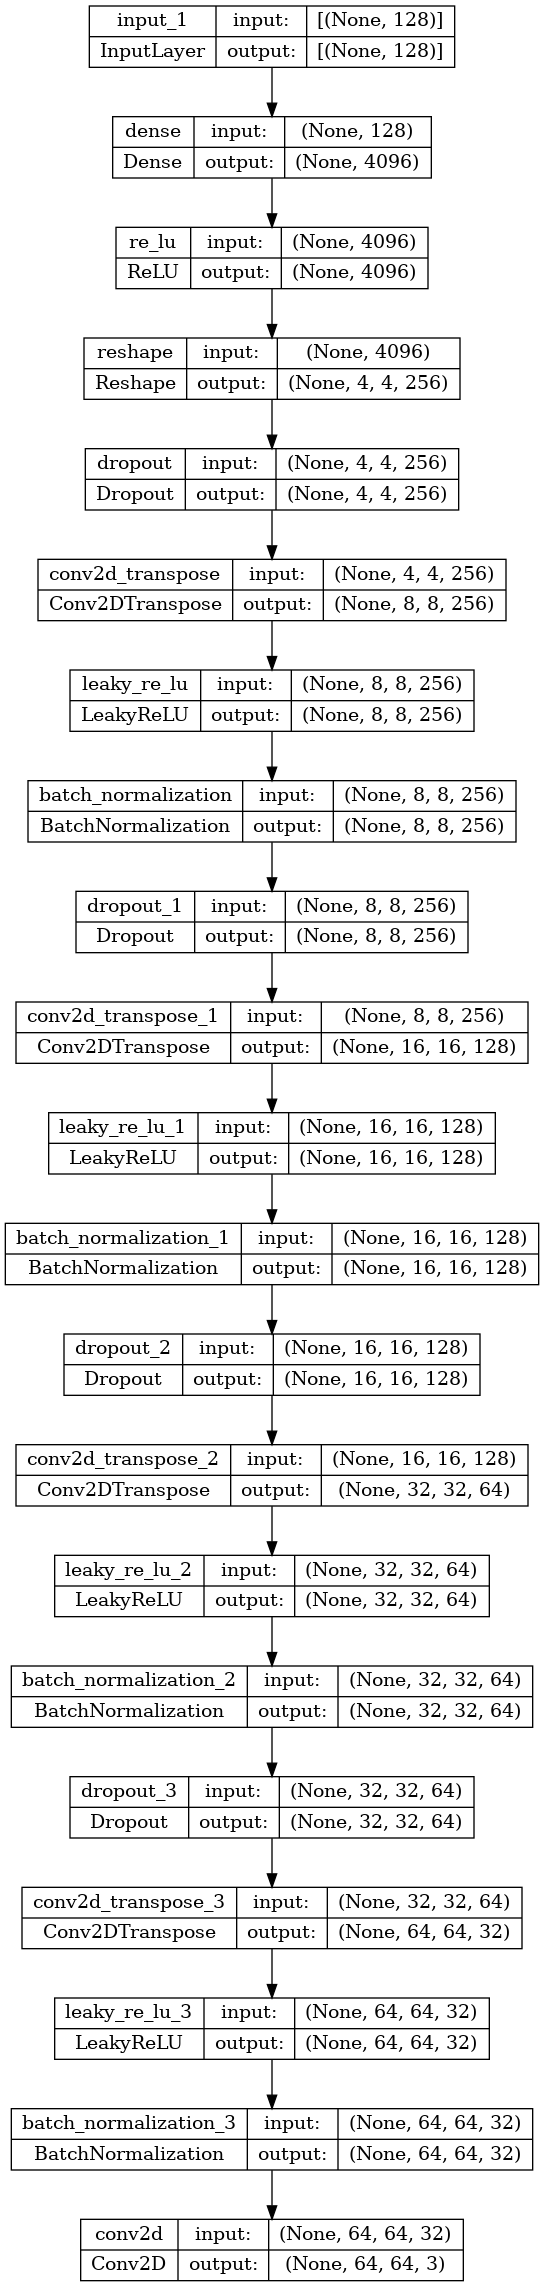
\includegraphics[width=.36\textwidth]{images/Generator.png}
    \centering
    \caption{Generator used for celebGAN}
\end{figure}

\subsection{Discriminator Plot}
\label{apx:dcgan_discriminator}
\begin{figure}[H]
    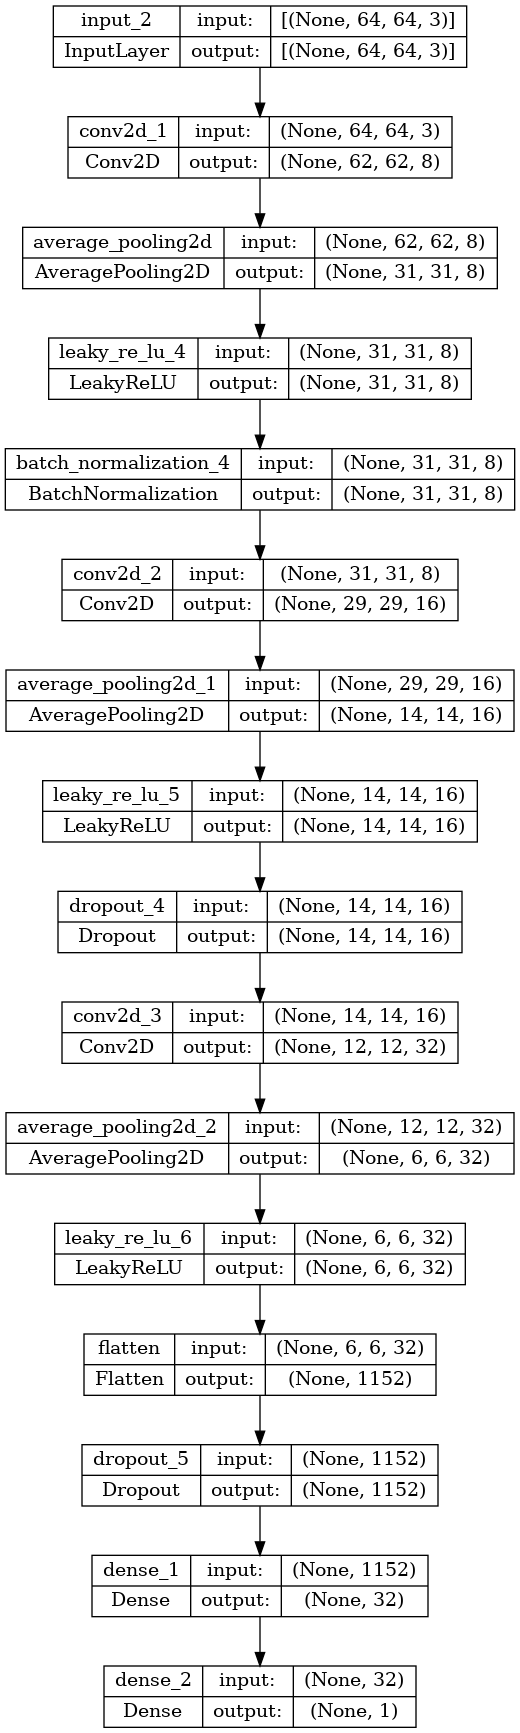
\includegraphics[width=.35\textwidth]{images/Discriminator.png}
    \centering
    \caption{Discriminator used for celebGAN}
\end{figure}

\subsection{Image Generation Code}
\label{apx:generation_code}
\begin{minted}
[
frame=lines,
framesep=2mm,
baselinestretch=1.2,
bgcolor=LightGray,
fontsize=\footnotesize,
linenos
]
{python}
import tensorflow as tf
import matplotlib.pyplot as plt
import numpy as np

generator = tf.keras.models.load_model('celebGAN/generator_model/generator.h5')

#for single image
lv = tf.random.normal([1, 128])
image = generator(lv)
imagenorm = image*127.5+127.5
imagenp = imagenorm.numpy()[0,:,:,:]
plt.imshow(imagenp.astype(dtype="int32"),
    interpolation='antialiased', interpolation_stage="rgba")

#for multiple images
images = 25
predictions = np.empty([100,64,64,3])
for i in range(4):
    seed = tf.random.normal([images, 128])
    label_seed = np.random.randint(0,2, images)
    pred = generator(seed, training=False).numpy()
    predictions[25*i:25*(i+1), :, :, :] = pred
    
print(predictions.shape)
figsize = 10
fig = plt.figure(figsize=(figsize, figsize))  
for i in range(predictions.shape[0]):
    plt.subplot(figsize, figsize, i+1)
    plt.imshow((predictions[i, :, :, :]*127.5+127.5).astype("int32"),
        interpolation='antialiased', interpolation_stage="rgba")
    plt.axis('off')
plt.show()
\end{minted}
\subsection{Loss for celebGAN2}
\label{apx:celebGAN2Loss}
\begin{figure}[H]
    \centering
    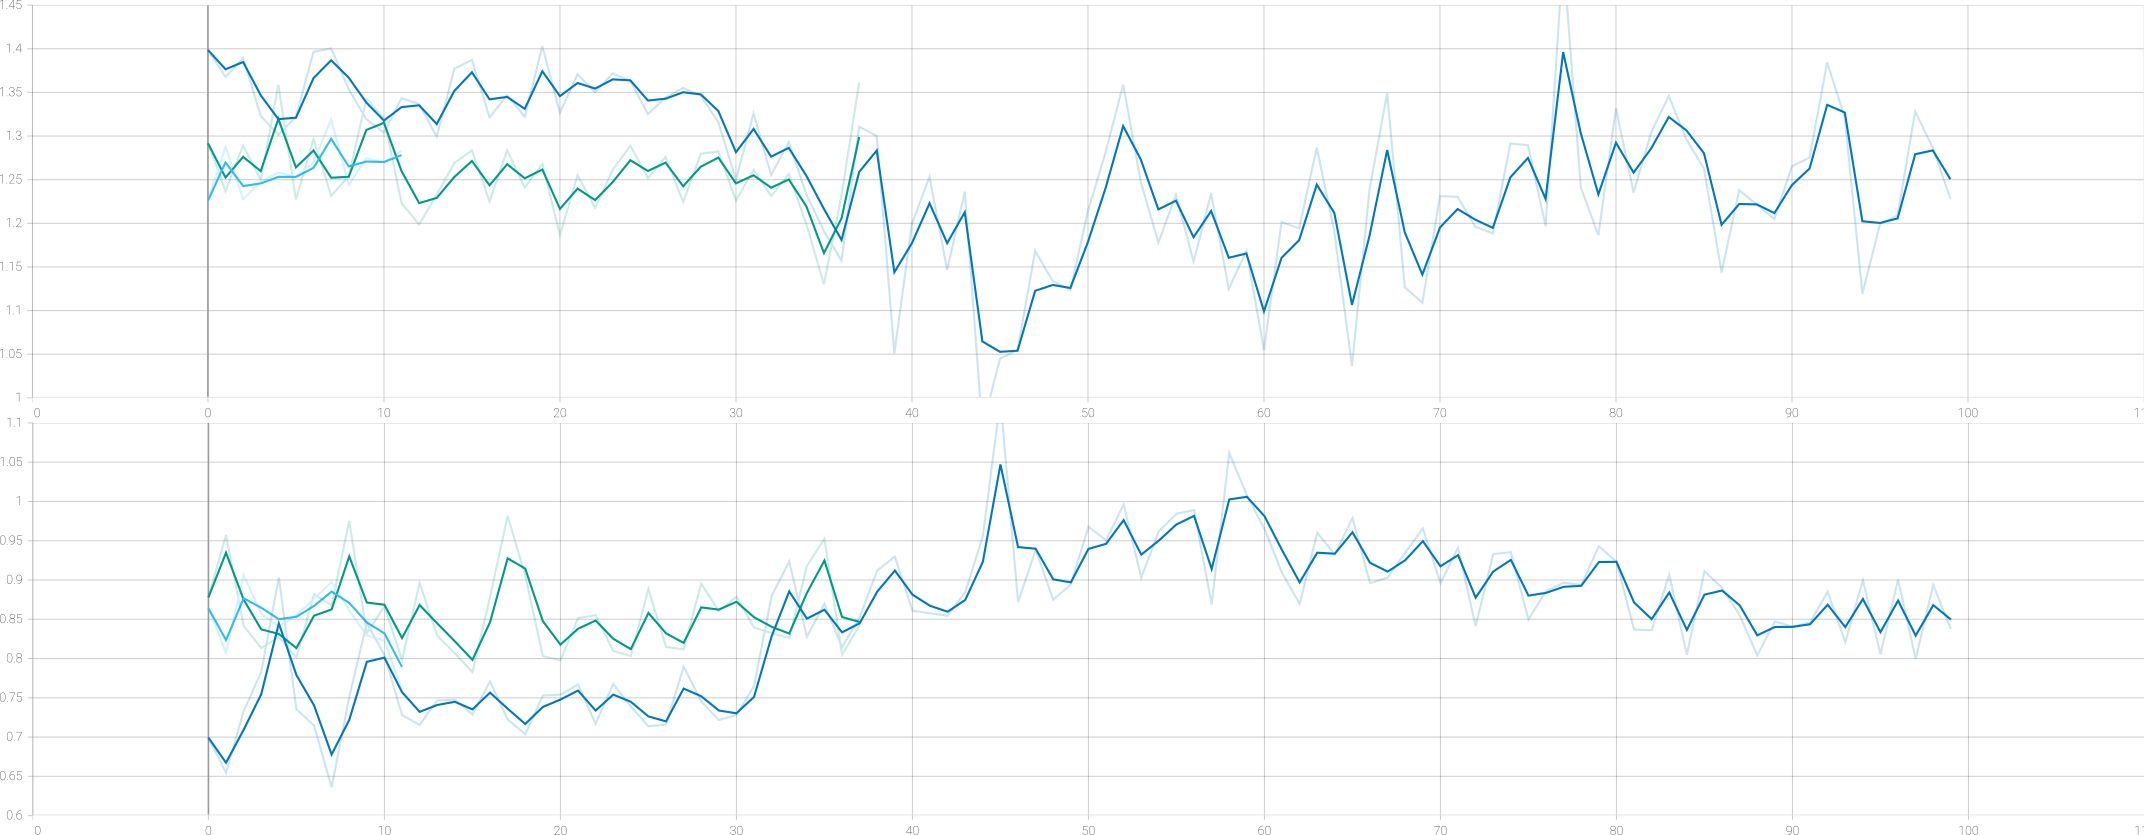
\includegraphics[width=0.9\textwidth]{images/BothLoss.png}
    \caption{\textbf{Top:} Discriminator Loss. \textbf{Bottom:} Generator Loss; Each line represents a training process at a different time}
    \label{fig:my_label}
\end{figure}

\section{Code}

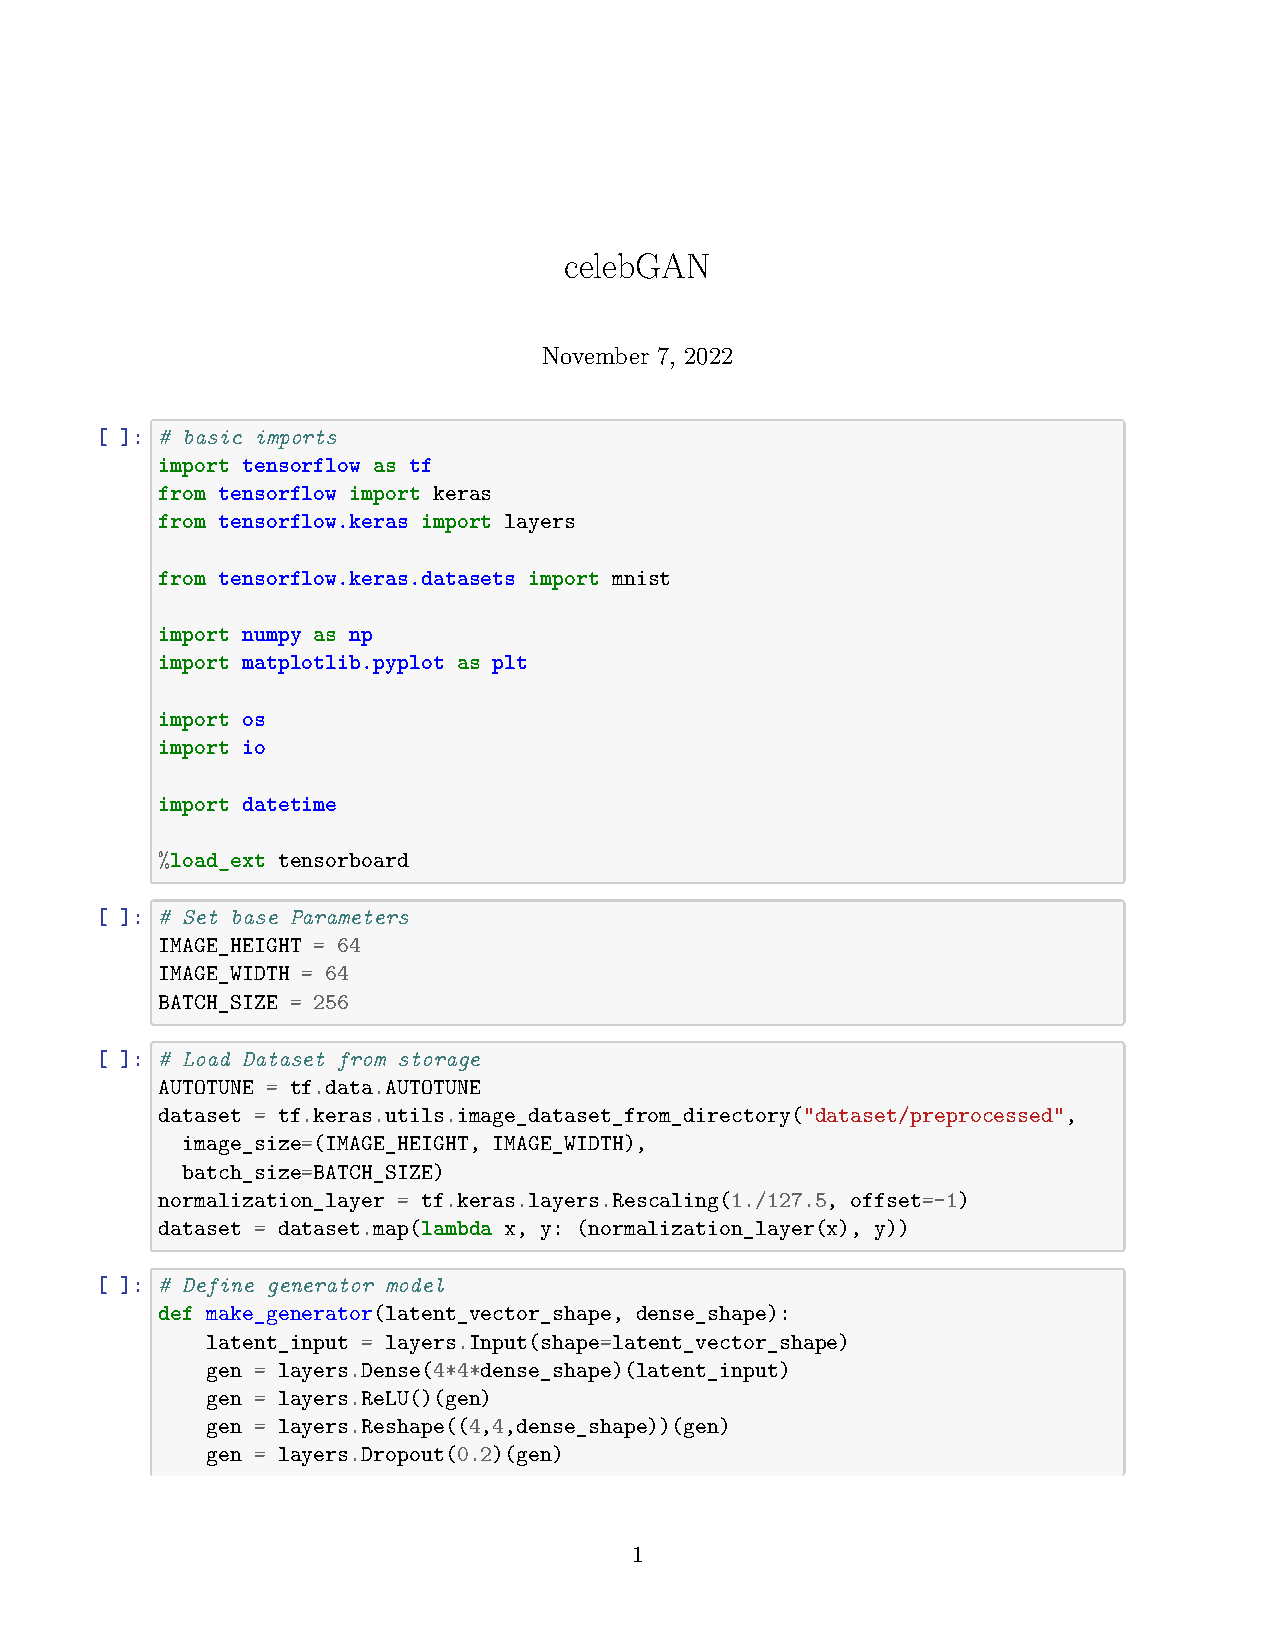
\includepdf[pages=-, addtotoc={1,subsection,2, celebGAN, apx:celebGAN}]{code/celebGAN.pdf}
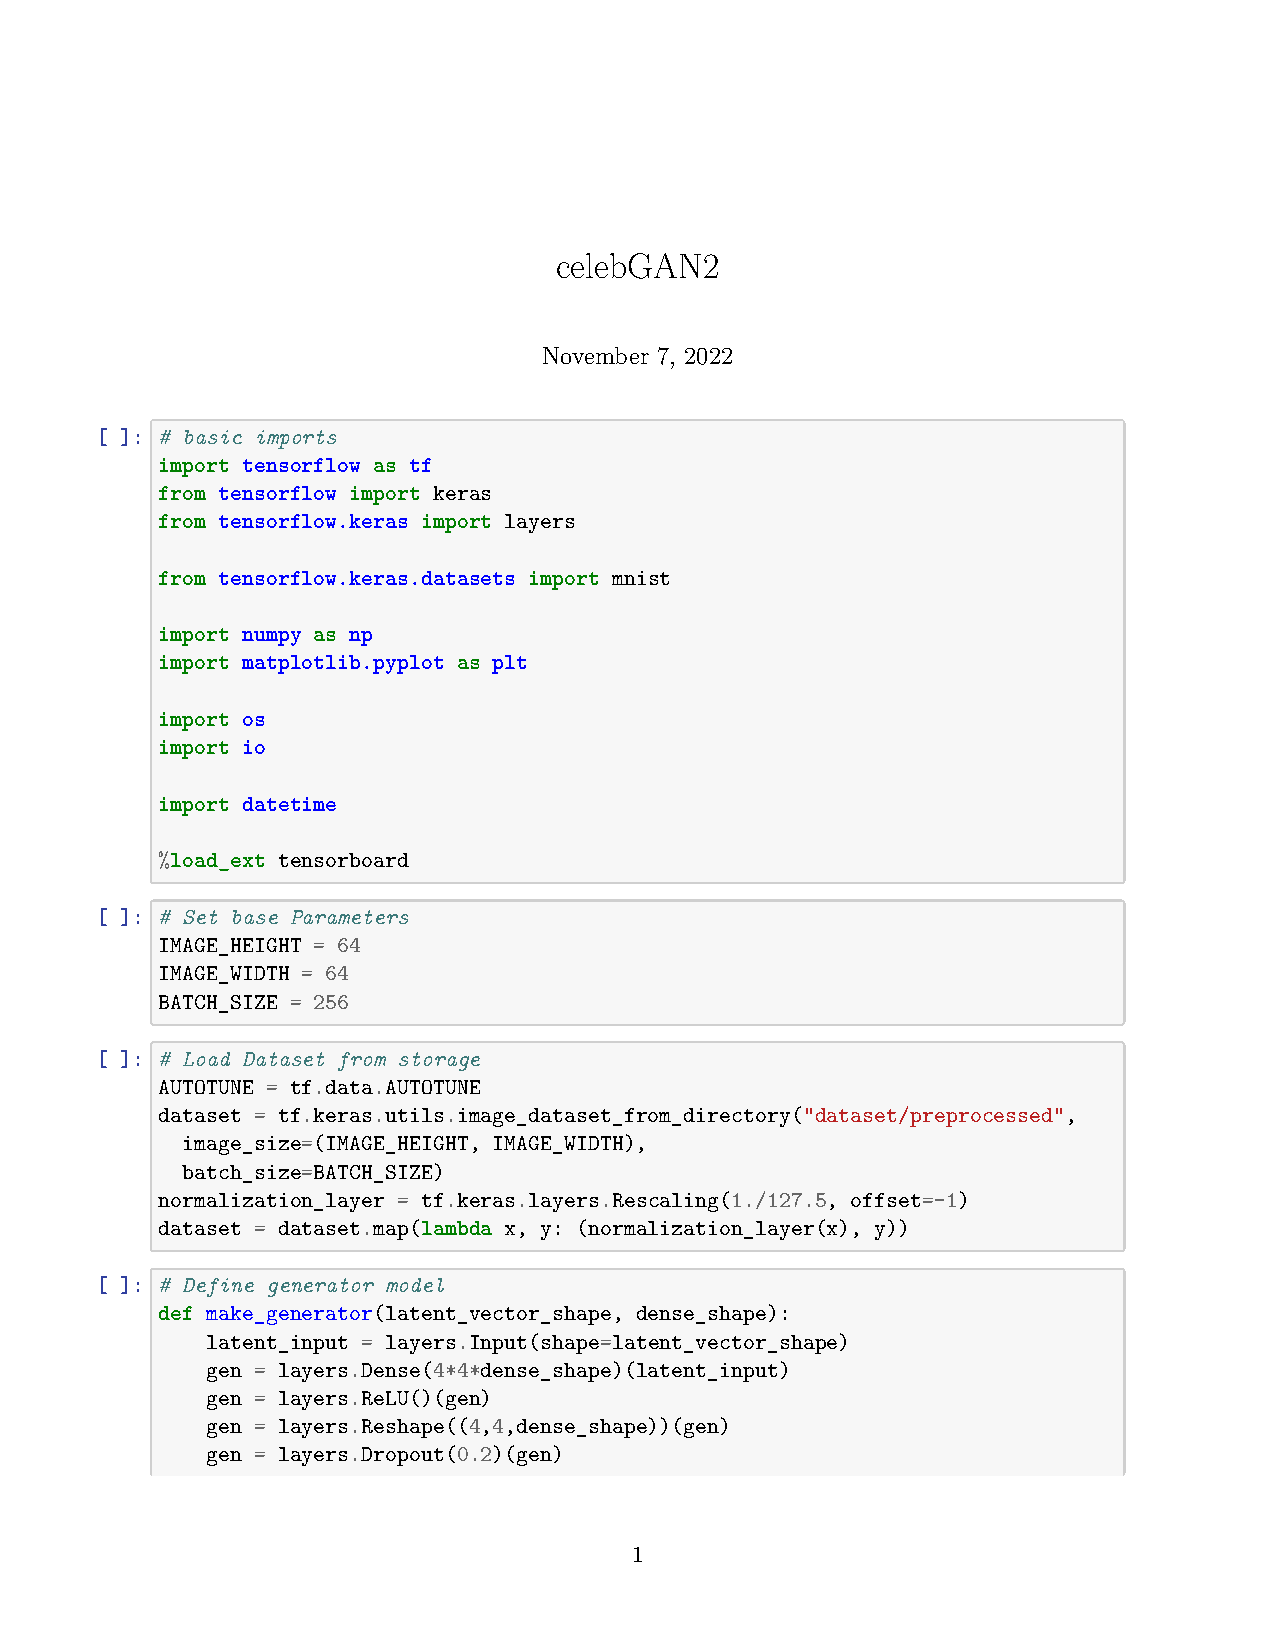
\includepdf[pages=-, addtotoc={1,subsection,2, celebGAN2, apx:celebGAN2}]{code/celebGAN2.pdf}
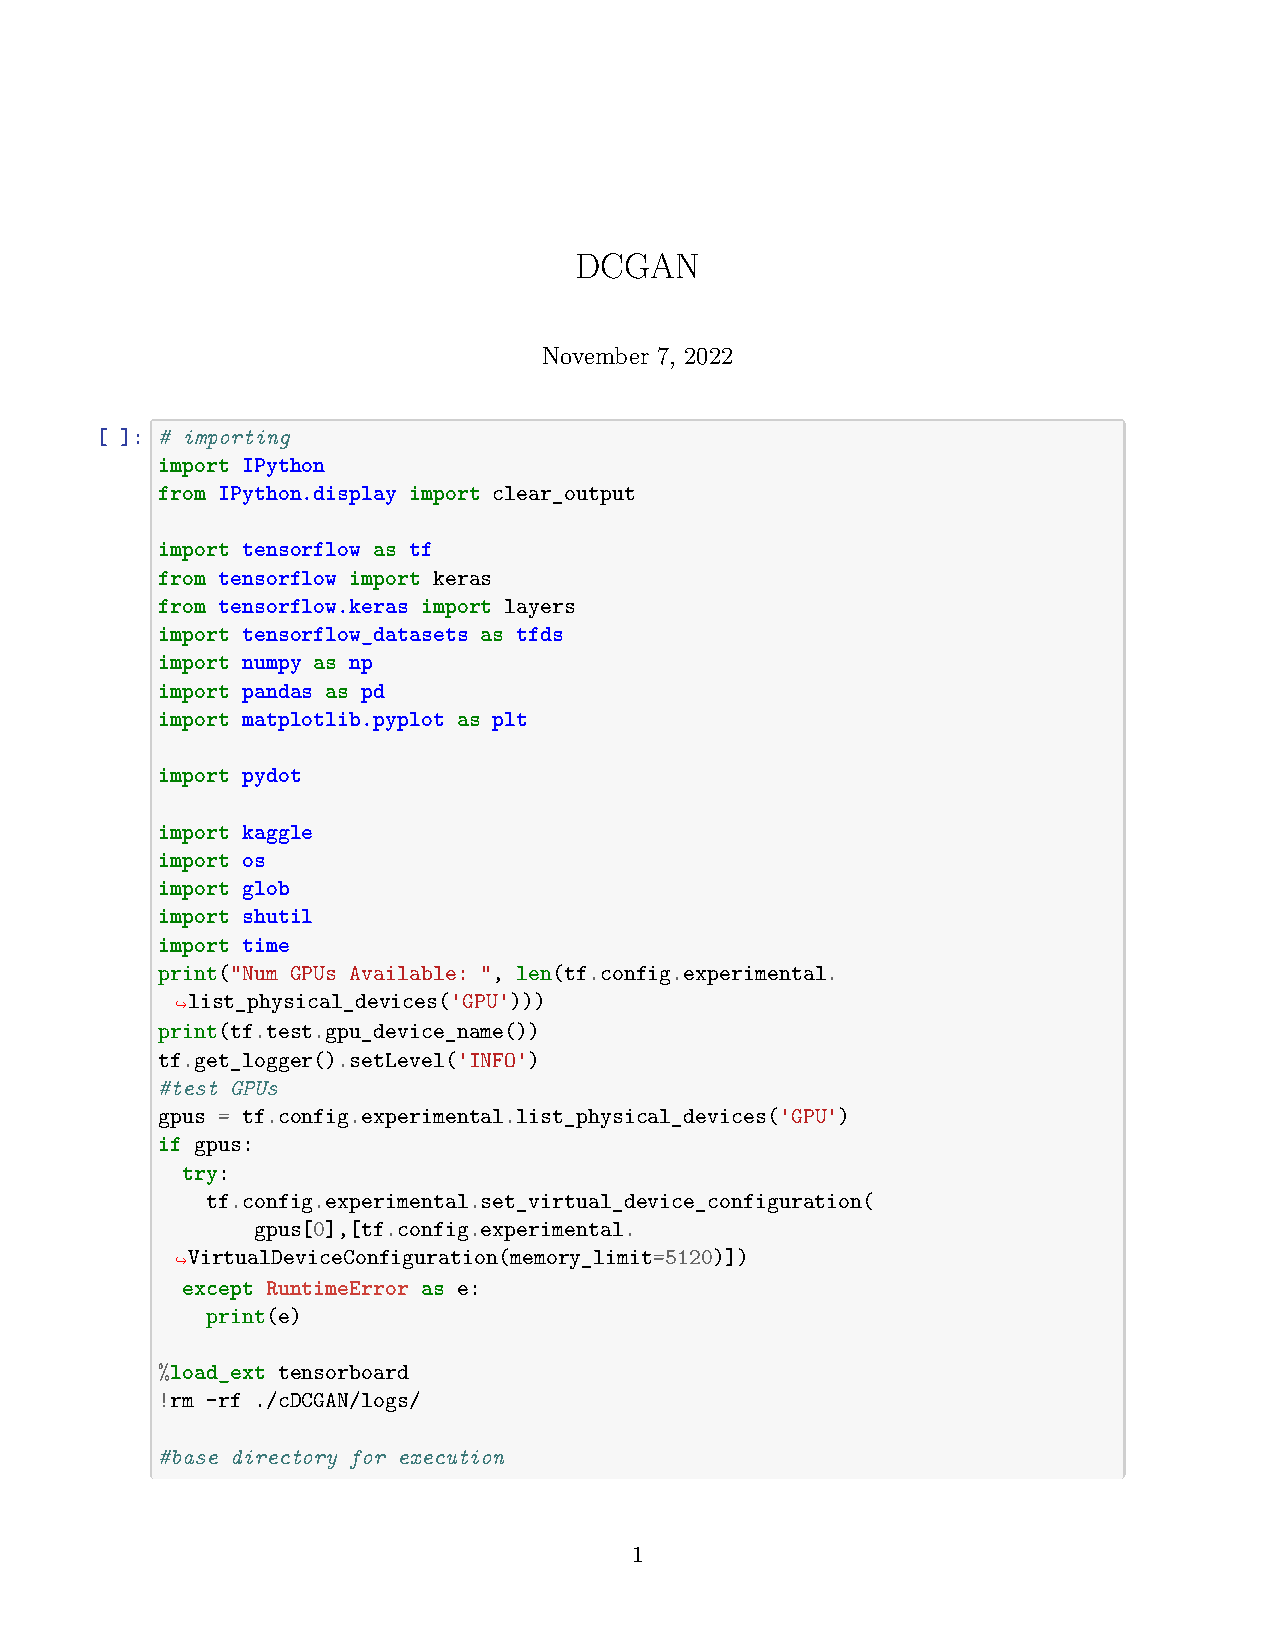
\includepdf[pages=-, addtotoc={1,subsection,2, DCGAN, apx:DCGAN}]{code/DCGAN.pdf}
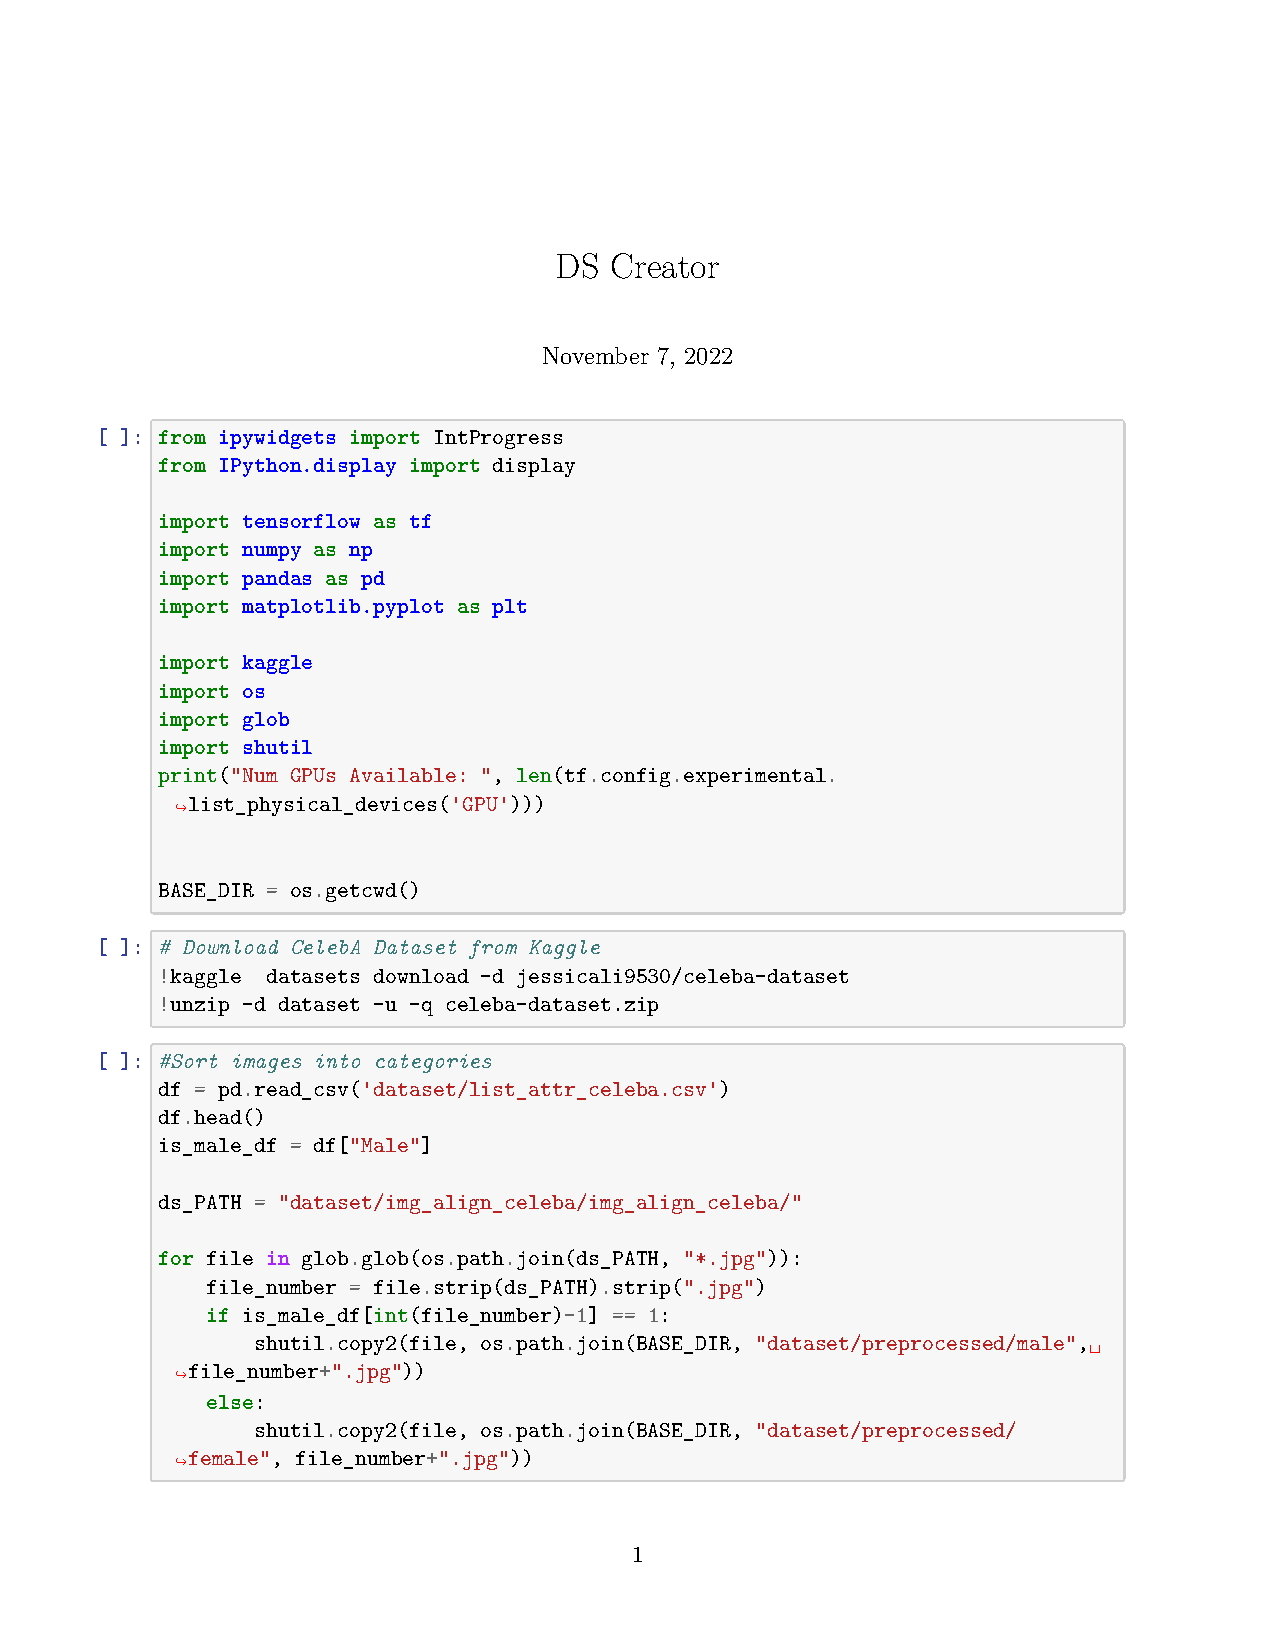
\includepdf[pages=-, addtotoc={1,subsection,2, Dataset Creator, apx:DS_Import}]{code/DSCreator.pdf}
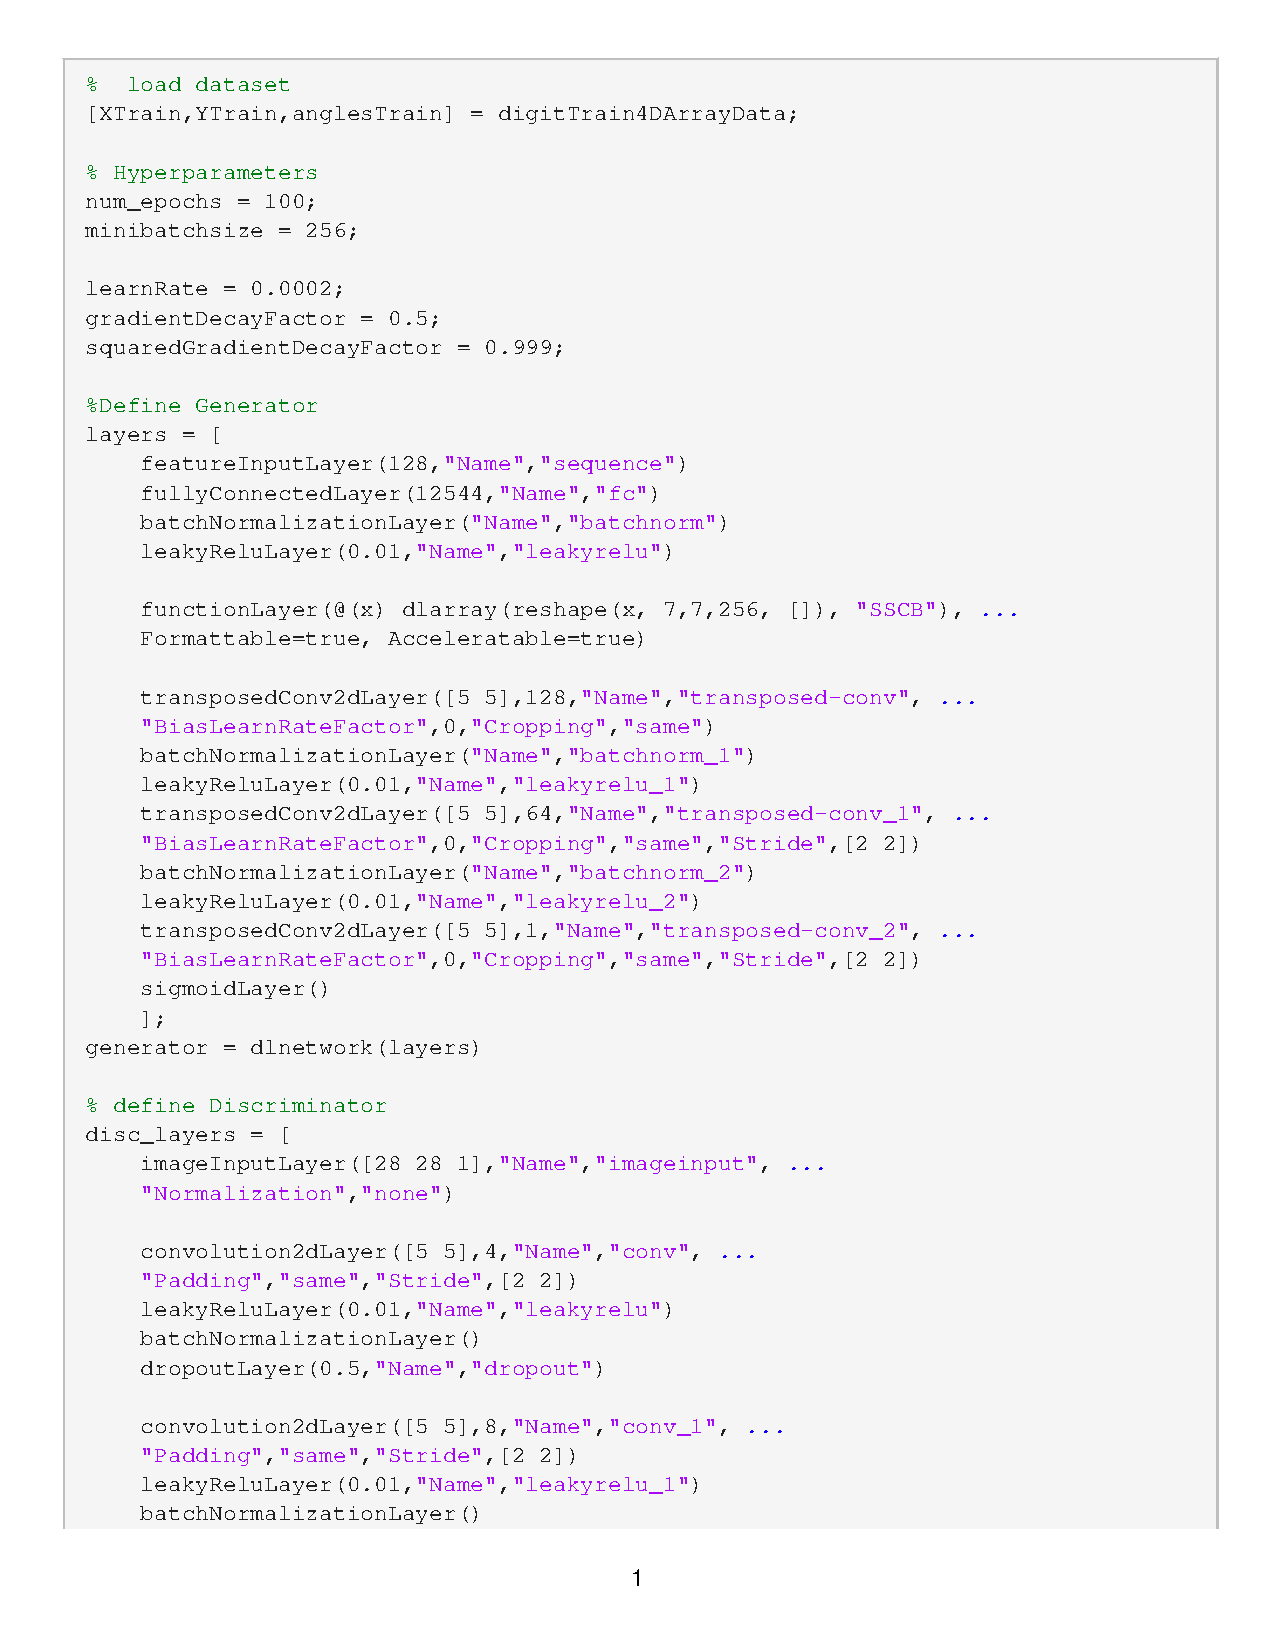
\includepdf[pages=-, addtotoc={1,subsection,2, Matlab GAN, apx:MLGAN}]{code/GAN.pdf}
\end{appendix}
